% THIS DOCUMENT IS TAILORED TO REQUIREMENTS FOR SCIENTIFIC COMPUTING.  IT SHOULDN'T
% BE USED FOR NON-SCIENTIFIC COMPUTING PROJECTS
\documentclass[12pt]{article}

\usepackage{amsmath, mathtools}
\usepackage{amsfonts}
\usepackage{amssymb}
\usepackage{graphicx}
\usepackage{colortbl}
\usepackage{xr}
\usepackage{hyperref}
\usepackage{longtable}
\usepackage{xfrac}
\usepackage{tabularx}
\usepackage{float}
\usepackage{siunitx}
\usepackage{booktabs}
\usepackage{caption}
\usepackage{pdflscape}
\usepackage{afterpage}
\usepackage{algpseudocode,algorithm}
\usepackage[inline,shortlabels]{enumitem}

\usepackage{tikz}
\usetikzlibrary{calc}
\usetikzlibrary{arrows}

\usepackage[backend=biber,style=authoryear]{biblatex}
\addbibresource{../../refs/References.bib}
%\usepackage{refcheck}

\hypersetup{
    bookmarks=true,         % show bookmarks bar?
    colorlinks=true,        % false: boxed links; true: colored links
    linkcolor=red,          % color of internal links (change box color with linkbordercolor)
    citecolor=green,        % color of links to bibliography
    filecolor=magenta,      % color of file links
    urlcolor=cyan           % color of external links
}

\input{../Comments}
%% Common Parts

\newcommand{\progname}{MPIR} % PUT YOUR PROGRAM NAME HERE
\newcommand{\authname}{Xunzhou (Joe) Ye} % AUTHOR NAMES

\newcommand{\matr}[1]{\mathbf{#1}}
\renewcommand{\vec}[1]{\mathbf{#1}}
\newcommand{\spann}[1]{\mathrm{span}\{#1\}}

\usepackage{hyperref}
    \hypersetup{colorlinks=true, linkcolor=blue, citecolor=blue, filecolor=blue,
                urlcolor=blue, unicode=false}
    \urlstyle{same}


% For easy change of table widths
\newcommand{\colZwidth}{1.0\textwidth}
\newcommand{\colAwidth}{0.13\textwidth}
\newcommand{\colBwidth}{0.82\textwidth}
\newcommand{\colCwidth}{0.1\textwidth}
\newcommand{\colDwidth}{0.05\textwidth}
\newcommand{\colEwidth}{0.8\textwidth}
\newcommand{\colFwidth}{0.17\textwidth}
\newcommand{\colGwidth}{0.5\textwidth}
\newcommand{\colHwidth}{0.28\textwidth}

% Used so that cross-references have a meaningful prefix
\newcounter{defnum} %Definition Number
\newcommand{\dthedefnum}{GD\thedefnum}
\newcommand{\dref}[1]{GD\ref{#1}}
\newcounter{datadefnum} %Datadefinition Number
\newcommand{\ddthedatadefnum}{DD\thedatadefnum}
\newcommand{\ddref}[1]{DD\ref{#1}}
\newcounter{datatypedefnum} %Data type definition Number
\newcommand{\ddthedatatypedefnum}{DT\thedatatypedefnum}
\newcommand{\dtref}[1]{DT\ref{#1}}
\newcounter{theorynum} %Theory Number
\newcommand{\tthetheorynum}{TM\thetheorynum}
\newcommand{\tref}[1]{TM\ref{#1}}
\newcounter{tablenum} %Table Number
\newcommand{\tbthetablenum}{TB\thetablenum}
\newcommand{\tbref}[1]{TB\ref{#1}}
\newcounter{assumpnum} %Assumption Number
\newcommand{\atheassumpnum}{A\theassumpnum}
\newcommand{\aref}[1]{A\ref{#1}}
\newcounter{goalnum} %Goal Number
\newcommand{\gthegoalnum}{GS\thegoalnum}
\newcommand{\gsref}[1]{GS\ref{#1}}
\newcounter{instnum} %Instance Number
\newcommand{\itheinstnum}{IM\theinstnum}
\newcommand{\iref}[1]{IM\ref{#1}}
\newcounter{reqnum} %Requirement Number
\newcommand{\rthereqnum}{R\thereqnum}
\newcommand{\rref}[1]{R\ref{#1}}
\newcounter{nfrnum} %NFR Number
\newcommand{\rthenfrnum}{NFR\thenfrnum}
\newcommand{\nfrref}[1]{NFR\ref{#1}}
\newcounter{lcnum} %Likely change number
\newcommand{\lthelcnum}{LC\thelcnum}
\newcommand{\lcref}[1]{LC\ref{#1}}

\usepackage{fullpage}

\newcommand{\deftheory}[9][Not Applicable]
{
\newpage
\noindent \rule{\textwidth}{0.5mm}

\paragraph{RefName: } \textbf{#2}
\refstepcounter{theorynum}
\phantomsection
\label{#2}

\paragraph{Label:} #3

\noindent \rule{\textwidth}{0.5mm}

\paragraph{Equation:}

#4

\paragraph{Description:}

#5

\paragraph{Notes:}

#6

\paragraph{Source:}

#7

\paragraph{Ref.\ By:}

#8

\paragraph{Preconditions for \hyperref[#2]{#2}:}
\label{#2_precond}

#9

\paragraph{Derivation for \hyperref[#2]{#2}:}
\label{#2_deriv}

#1

\noindent \rule{\textwidth}{0.5mm}

}

\begin{document}

\title{Software Requirements Specification for \progname: A Sparse Linear Solver}
\author{\authname}
\date{\today}

\maketitle

~\newpage

\pagenumbering{roman}

\tableofcontents

~\newpage

\section*{Revision History}

\begin{tabularx}{\textwidth}{p{3cm}p{2cm}X}
  \toprule {\bf Date}    & {\bf Version} & {\bf Notes}                                     \\
  \midrule
  \date{26 January 2025} & 1.0           & Initial draft                                   \\
  \date{26 March 2025}   & 1.1           & Updates regarding peer and instructor feedbacks \\
  \bottomrule
\end{tabularx}

~\newpage

\section{Reference Material}

This section records information for easy reference.

\subsection{Table of Units}

Not applicable to this project because it does not interact with any physical
system.

\subsection{Table of Symbols}

The table that follows summarizes the symbols used in this document. The choice
of symbols was made to be consistent with common numerical computing
literatures.

\renewcommand{\arraystretch}{1.2}
\noindent \begin{longtable*}{l p{12cm}}
  \toprule
  \textbf{symbol}    & \textbf{description} \\
  \midrule
  \(n\)        & The size of a vector/matrix \\
  \(\matr{A}\) & An \(n \times n\) matrix to be solved \\
  \(\vec{b}\)        & Some \(n\)-vector \\
  \(\epsilon\)        & a solution is found if the norm of the residual is less than \(\epsilon\) \\
  \(n_\mathrm{iter}\) & the maximum number of iterations to perform \\
  \(u_f\)       & factorization precision \\
  \(u_w\)       & working precision \\
  \(u_r\)       & precision in which the residuals are computed \\
  \bottomrule
\end{longtable*}

\subsection{Abbreviations and Acronyms}

\renewcommand{\arraystretch}{1.2}
\begin{tabular}{l l}
  \toprule
  \textbf{symbol} & \textbf{description} \\
  \midrule
  A         & Assumption \\
  DD        & Data Definition \\
  GD        & General Definition \\
  GMRES     & General Minimal Residual Method \\
  GS        & Goal Statement \\
  IM        & Instance Model \\
  IR        & Iterative refinement \\
  LC        & Likely Change \\
  MP        & Mixed-precision \\
  PS        & Physical System Description \\
  R         & Requirement \\
  SRS       & Software Requirements Specification \\
  TM        & Theoretical Model \\
  \bottomrule
\end{tabular}

\subsection{Mathematical Notation}

\plt{This section is optional, but should be included for projects that make use
  of notation to convey mathematical information.  For instance, if typographic
  conventions (like bold face font) are used to distinguish matrices, this
  should be stated here.  If symbols are used to show mathematical operations,
  these should be summarized here.  In some cases the easiest way to summarize
  the notation is to point to a text or other source that explains the
  notation.}

\plt{This section was added to the template because some students use very
  domain specific notation.  This notation will not be readily understandable to
  people outside of your domain.  It should be explained.}

This document annotates variables of matrices or vectors in math bold face. For
any matrix \(\matr{A}\) or vector \(\vec{b}\), one with subscript \(\matr{A}_i\)
or \(\vec{b}_i\) always means ``the \(i\)th matrix/vector''. \(a_{i,j}\) or
\(b_{i}\) is used to reference ``the element at row \(i\) column \(j\) in matrix
\(\matr{A}\)'' or ``the \(i\)th element in vector \(\vec{b}\)''.

\newpage

\pagenumbering{arabic}

\plt{The SRS is not generally written, or read, sequentially.  The SRS is a
  reference document.  It is generally read in an ad hoc order, as the need
  arises.  For writing an SRS, and for reading one for the first time, the
  suggested order of sections is:
\begin{itemize}
\item Goal Statement
\item Instance Models
\item Requirements
\item Introduction
\item Specific System Description
\end{itemize}
}

\plt{Guiding principles for the SRS document:
\begin{itemize}
\item Do not repeat the same information at the same abstraction level.  If
  information is repeated, the repetition should be at a different abstraction
  level.  For instance, there will be overlap between the scope section and the
  assumptions, but the scope section will not go into as much detail as the
  assumptions section.
\end{itemize}
}

\plt{The template description comments should be disabled before submitting this
  document for grading.}

\plt{You can borrow any wording from the text given in the template.  It is part
  of the template, and not considered an instance of academic integrity.  Of
  course, you need to cite the source of the template.}

\plt{When the documentation is done, it should be possible to trace back to the
  source of every piece of information.  Some information will come from
  external sources, like terminology.  Other information will be derived, like
  General Definitions.}

\plt{An SRS document should have the following qualities: unambiguous,
  consistent, complete, validatable, abstract and traceable.}

\plt{The overall goal of the SRS is that someone that meets the Characteristics
  of the Intended Reader (Section~\ref{sec_IntendedReader}) can learn,
  understand and verify the captured domain knowledge.  They should not have to
  trust the authors of the SRS on any statements.  They should be able to
  independently verify/derive every statement made.}

\section{Introduction}

Solving linear systems is a key part of numerical computing and is widely used
in many applications, creating a demand for fast and reliable solvers. Modern
hardware and software have shown that using lower-precision calculations can be
much faster and more memory-efficient than traditional double-precision (64-bit)
methods. Mixed-precision (MP) algorithms combine the speed of lower-precision
calculations with the accuracy of higher-precision ones to improve performance
in various linear solvers. The document describes the solver called \progname,
which implements an iterative method in mixed-precisions and uses General
Minimal RESidual (GMRES) in particular for find the error correction vector
during the refinement process.

The following section provides an overview of the Software Requirements
Specification (SRS) for \progname. This section explains the purpose of this
document, the scope of the requirements, the characteristics of the intended
reader, and the organization of the document.

\subsection{Purpose of Document}

\plt{This section summarizes the purpose of the SRS document.  It does not focus
  on the problem itself.  The problem is described in the ``Problem
  Description'' section (Section~\ref{Sec_pd}).  The purpose is for the document
  in the context of the project itself, not in the context of this course.
  Although the ``purpose'' of the document is to get a grade, you should not
  mention this.  Instead, ``fake it'' as if this is a real project.  The purpose
  section will be similar between projects.  The purpose of the document is the
  purpose of the SRS, including communication, planning for the design stage,
  etc.}

The primary purpose of this document is to record the requirements of \progname.
Goals, assumptions, theoretical models, definitions, and other model derivation
information are specified, allowing the reader to fully understand and verify
the purpose and scientific basis of \progname.

\subsection{Scope of Requirements}

\plt{Modelling the real world requires simplification.  The full complexity of
  the actual physics, chemistry, biology is too much for existing models, and
  for existing computational solution techniques.  Rather than say what is in
  the scope, it is usually easier to say what is not.  You can think of it as
  the scope is initially everything, and then it is constrained to create the
  actual scope.  For instance, the problem can be restricted to 2 dimensions, or
  it can ignore the effect of temperature (or pressure) on the material
  properties, etc.}

\plt{The scope section is related to the assumptions section
  (Section~\ref{sec_assumpt}).  However, the scope and the assumptions are not
  at the same level of abstraction.  The scope is at a high level.  The focus is
  on the ``big picture'' assumptions.  The assumptions section lists, and
  describes, all of the assumptions.}

\plt{The scope section is relevant for later determining typical values of
  inputs. The scope should make it clear what inputs are reasonable to expect.
  This is a distinction between scope and context (context is a later section).
  Scope affects the inputs while context affects how the software will be used.}

The scope of the software is limited to solving sparse real matrices. For
completeness of the software suite, an example program for demonstrating the use
of the core solver should be also considered. In terms of writing the
requirement specifications itself, operational specifications will be given at a
high level without expanding into details on each and every mathematical terms.

\subsection{Characteristics of Intended Reader} \label{sec_IntendedReader}

\plt{This section summarizes the skills and knowledge of the readers of the
  SRS.  It does NOT have the same purpose as the ``User Characteristics''
  section (Section~\ref{SecUserCharacteristics}).  The intended readers are the
  people that will read, review and maintain the SRS.  They are the people that
  will conceivably design the software that is intended to meet the
  requirements.  The user, on the other hand, is the person that uses the
  software that is built.  They may never read this SRS document.  Of course,
  the same person could be a ``user'' and an ``intended reader.''}

\plt{The intended reader characteristics should be written as unambiguously and
  as specifically as possible.  Rather than say, the user should have an
  understanding of physics, say what kind of physics and at what level.  For
  instance, is high school physics adequate, or should the reader have had a
  graduate course on advanced quantum mechanics?}

The intended reader of this document is expected to have a strong foundation in
linear algebra at the undergraduate level, with a preference for those who
possess graduate-level knowledge in numerical analysis and linear solvers. At a
minimum, readers should have completed an introductory undergraduate course in
linear algebra and scientific computing, such as MATH 1ZC3 (Linear Algebra) and
SFWRENG 4X03 (Scientific Computing) at McMaster University, or equivalent
courses from another institution. This background ensures that readers can
effectively understand and evaluate the mathematical formulations, algorithmic
considerations, and numerical techniques described in this document.

\subsection{Organization of Document}

The organization of this document follows the template for an SRS for scientific
computing software. The presentation follows the standard pattern of presenting
goals, theories, definitions, and assumptions. For readers that would like a
more bottom up approach, they can start reading the instance models and trace
back to find any additional information they require.

The goal statements are refined to the theoretical models and the theoretical
models to the instance models.

\section{General System Description}

This section provides general information about the system.  It identifies the
interfaces between the system and its environment, describes the user
characteristics and lists the system constraints.

\plt{The purpose of this section is to provide general information about the
  system so the specific requirements in the next section will be easier to
  understand. The general system description section is designed to be
  changeable independent of changes to the functional requirements documented in
  the specific system description. The general system description provides a
  context for a family of related models.  The general description can stay the
  same, while specific details are changed between family members.}

\subsection{System Context}

\plt{Your system context will include a figure that shows the abstract view of
  the software.  Often in a scientific context, the program can be viewed
  abstractly following the design pattern of Inputs $\rightarrow$ Calculations
  $\rightarrow$ Outputs.  The system context will therefore often follow this
  pattern.  The user provides inputs, the system does the calculations, and then
  provides the outputs to the user.  The figure should not show all of the
  inputs, just an abstract view of the main categories of inputs (like material
  properties, geometry, etc.).  Likewise, the outputs should be presented from
  an abstract point of view.  In some cases the diagram will show other external
  entities, besides the user.  For instance, when the software product is a
  library, the user will be another software program, not an actual end user.
  If there are system constraints that the software must work with external
  libraries, these libraries can also be shown on the System Context diagram.
  They should only be named with a specific library name if this is required by
  the system constraint.}

\begin{figure}[h!]
  \centering
  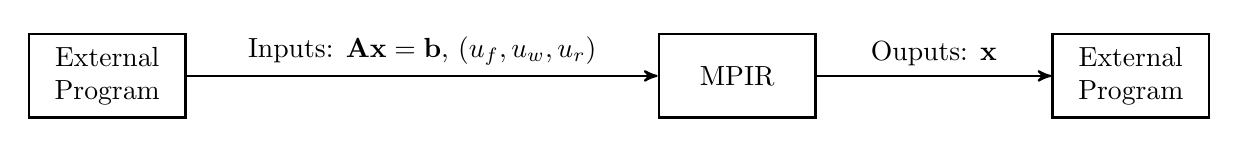
\begin{tikzpicture}[%
    auto,
    block/.style={
      rectangle,
      draw=black,
      thick,
      text width=5em,
      align=center,
      minimum height=3em
    },
    thick,
    >=stealth'
    ]
    \draw (-8,0) node[block] (ex1) {External Program};
    \draw (0,0) node[block] (sys) {\progname{}};
    \draw (5,0) node[block] (ex2) {External Program};

    \draw [->] (ex1) -- (sys) node[midway,above] () {Inputs: \(\matr{A}\vec{x} = \vec{b}\), \((u_f, u_w, u_r)\)};
    \draw [->] (sys) -- (ex2) node[midway,above] () {Ouputs: \(\vec{x}\)};
  \end{tikzpicture}
  \caption{System Context}
  \label{Fig_SystemContext}
\end{figure}

\plt{For each of the entities in the system context diagram its responsibilities
  should be listed.  Whenever possible the system should check for data quality,
  but for some cases the user will need to assume that responsibility.  The list
  of responsibilities should be about the inputs and outputs only, and they
  should be abstract.  Details should not be presented here.  However, the
  information should not be so abstract as to just say ``inputs'' and
  ``outputs''.  A summarizing phrase can be used to characterize the inputs.
  For instance, saying ``material properties'' provides some information, but it
  stays away from the detail of listing every required properties.}

\begin{itemize}
\item User Responsibilities:
  \begin{itemize}
  \item Provide a sparse matrix \(\matr{A}: \mathbb{R}^{n \times n}\) in Compressed Sparse Column
    (CSC) format (\cite{noauthor_compressed_nodate}) stored in memory with
    appropriate data type.
  \item Provide an/multiple vector(s) \(\vec{b}: \mathbb{R}^n\) to be solved for.
  \item Specify 3 floating point arithmetics precisions \((u_f, u_w, u_r)\) in which
    factorization, numeric solves, and residual computation will be performed
    respectively.
  \item Ensure \(\matr{A}\) satisfies the system assumption \aref{A:quasi}.
  \end{itemize}
\item \progname{} Responsibilities:
  \begin{itemize}
  \item Numerically solve \(\vec{x}\) for \(\matr{A}\vec{x} = \vec{b}\).
  \end{itemize}
\end{itemize}

\plt{Identify in what context the software will typically be used.  Is it for
exploration? education? engineering work? scientific work?. Identify whether it
will be used for mission-critical or safety-critical applications.} \plt{This
additional context information is needed to determine how much effort should be
devoted to the rationale section.  If the application is safety-critical, the
bar is higher.  This is currently less structured, but analogous to, the idea to
the Automotive Safety Integrity Levels (ASILs) that McSCert uses in their
automotive hazard analyses.}

\subsection{User Characteristics} \label{SecUserCharacteristics}

The end user of \progname{} is typically a technically proficient, domain-expert
professional or researcher who is focused on solving large-scale, sparse linear
systems efficiently. Users often come from fields such as computational physics,
engineering, computer science, applied mathematics, or data science, where large
sparse linear systems arise naturally (e.g., from discretized PDEs, network
analysis, or optimization problems). They work with problems that are too large
or complex for direct solvers, often involving millions or billions of unknowns.
The user should also be proficient in programming languages commonly used for
numeric analysis and high performance computing such as MATLAB, C/C++, or
Fortran. They should have a strong understanding of floating point numbers
representations as well as the pitfalls in floating point arithmetics in modern
computers. This is especially needed to configure the inputs for the software.
At a minimum, the user should have completed an introductory undergraduate
course in scientific computing, such as SFWRENG 4X03 (Scientific Computing) at
McMaster University, or equivalent courses from another institution.

\subsection{System Constraints}

This project is based on existing research with the intent to develop on top of
the existing implementation of a solver with similar functionalities. This
places constraints:

\begin{enumerate}
\item Internal matrix solves must use the Generalized Minimal RESidual (GMRES)
  method (\cite{lindquist_improving_2020}).
\end{enumerate}

\section{Specific System Description}

This section first presents the problem description, which gives a high-level
view of the problem to be solved.  This is followed by the solution characteristics
specification, which presents the assumptions, theories, definitions and finally
the instance models.  \plt{Add any project specific details that are relevant
  for the section overview.}

\subsection{Problem Description} \label{Sec_pd}

\progname{} is a solver intended to find a numerical solution \(\vec{x}\) to a sparse
linear system characterized in the equation \(\matr{A}\vec{x} = \vec{b}\), where
\(\matr{A}\) is an \(n \times n\) matrix and \(\vec{b}\) is an \(n\) vector.

\subsubsection{Terminology and Definitions}

\plt{This section is expressed in words, not with equations.  It provide the
  meaning of the different words and phrases used in the domain of the problem.
The terminology is used to introduce concepts from the world outside of the
mathematical model  The terminology provides a real world connection to give the
mathematical model meaning.}

% This subsection provides a list of terms that are used in the subsequent
% sections and their meaning, with the purpose of reducing ambiguity and making it
% easier to correctly understand the requirements:

% \begin{itemize}
% \item
% \end{itemize}

Text descriptions are included along with their mathematical definitions as most
of the terms used in this document is about math and linear algebra.


\subsubsection{Physical System Description} \label{sec_phySystDescrip}

Not applicable to this project because it does not interact with any physical
system.

\subsubsection{Goal Statements}

\noindent Given an \(n \times n\) matrix \(\matr{A}\) and an \(n\) vector \(\vec{b}\),
where \(n\) is the size of the matrix, the goal statement is:

\begin{itemize}
\item[GS\refstepcounter{goalnum}\thegoalnum \label{GS:Axb}:] find a numerical
  solution \(\vec{x}\) to the linear system characterized in the equation
  \(\matr{A}\vec{x} = \vec{b}\).
\end{itemize}

\subsection{Solution Characteristics Specification}

This section specifies the information in the solution domain of \progname. This
section is intended to express what is required in such a way that analysts and
stakeholders get a clear picture, and the latter will accept it. The purpose of
this section is to reduce the problem into one expressed in mathematical terms.

This section presents the solution characteristics by successively refining
models. It starts with the abstract/general Theoretical Models (TMs) and refines
them to the concrete/specific Instance Models (IMs). The instance models that
govern \progname are presented in Subsection~\ref{sec_instance}. The
information to understand the meaning of the instance models and their
derivation is also presented, so that the instance models can be verified.

\subsubsection{Types}

\plt{This section is optional. Defining types can make the document easier to
understand.}

Optionally omitted.

\subsubsection{Scope Decisions}

The scope of this project is inherently limited due to the need to build upon a
prior research work (\cite{wong_exploring_2024}) rather than formulating a
completely new approach to the problem described in Section \ref{Sec_pd}. A
signification portion of this project is dedicated to refactor the prior work,
ensuring consistency with its methodology and results before introducing any new
contributions. This project must adhere to the same assumptions established in
the original study to maintain comparability and validity, as altering these
assumptions would fundamentally change the research direction. These assumptions
are listed in detail in Section~\ref{sec_assumpt}.

\subsubsection{Modelling Decisions}

\plt{This section is optional.}

Optionally omitted.

\subsubsection{Assumptions} \label{sec_assumpt}

\plt{The assumptions are a refinement of the scope.  The scope is general, where
  the assumptions are specific.  All assumptions should be listed, even those
  that domain experts know so well that they are rarely (if ever) written down.}
\plt{The document should not take for granted that the reader knows which
  assumptions have been made. In the case of unusual assumptions, it is
  recommended that the documentation either include, or point to, an explanation
  and justification for the assumption.}
\plt{If it helps with the organization and understandability, the assumptions
can be presented as sub sections.  The following sub-sections are options:
background theory assumptions, helper theory assumptions, generic theory
assumptions, problem specific assumptions, and rationale assumptions}

This section simplifies the original problem and helps in developing the
theoretical model by filling in the missing information for the physical system.
The numbers given in the square brackets refer to the theoretical model [TM],
general definition [GD], data definition [DD], instance model [IM], or likely
change [LC], in which the respective assumption is used.

\begin{itemize}
\item[A\refstepcounter{assumpnum}\theassumpnum \label{A:quasi}:] The input matrix
  \(\matr{A}\) is non-singular and symmetric quasi-definite \footnote{Definitions of
  symmetric matrices and quasi-definite matrices are given in \ddref{DD:sym} and
  \ddref{DD:quasidef}, respectively.}. [\tref{TM:LDL}]
\item[A\refstepcounter{assumpnum}\theassumpnum \label{A:prec}:] The given
  precisions follow the order \(u_f \leq u_w \leq u_r\), with \(u_r\) being the
  highest precision. [\tref{TM:IR}]

  \plt{Short description of each assumption. Each assumption
    should have a meaningful label. Use cross-references to identify the
    appropriate traceability to TM, GD, DD etc., using commands like dref, ddref
    etc. Each assumption should be atomic - that is, there should not be an
    explicit (or implicit) ``and'' in the text of an assumption.}

\end{itemize}

\subsubsection{Theoretical Models}\label{sec_theoretical}

\plt{Theoretical models are sets of abstract mathematical equations or axioms
  for solving the problem described in Section ``Physical System Description''
  (Section~\ref{sec_phySystDescrip}). Examples of theoretical models are
  physical laws, constitutive equations, relevant conversion factors, etc.}

\plt{Optionally the theory section could be divided into subsections to provide
more structure and improve understandability and reusability.  Potential
subsections include the following: Context theories, background theories, helper
theories, generic theories, problem specific theories, final theories and
rationale theories.}

This section focuses on the general equations and laws that \progname{} is based
on.  \plt{Modify the examples below for your problem, and add additional models
  as appropriate.}

~\newline

\noindent
\deftheory
% #2 refname of theory
{TM:LDL}
% #3 label
{\(\matr{L}\matr{D}\matr{L}\transpose\) factorization}
% #4 equation
{\(\matr{P}\matr{K}\matr{P}\transpose = \matr{L}\matr{D}\matr{L}\transpose\)}
% #5 description
{ Symmetric quasi-definite matrices are strongly factorizable. For any
  permutation \(\matr{P}\) of some symmetric quasi-definite matrix \(\matr{K}\),
  there is a diagonal \(\matr{D}\) and a unit
  lower-triangular \(\matr{L}\) such that the above equation holds. \\
  Under Assumption~\aref{A:quasi}, the input matrix \(\matr{A}\) can always be
  decomposed into \(\matr{L}\matr{D}\matr{L}\transpose\) factors, regardless of
  whether it is permuted.}
% #6 Notes
{ Definitions of symmetric matrices and quasi-definite matrices are given in
  \ddref{DD:sym} and \ddref{DD:quasidef}, respectively. In general, if factors
  are obtained for some matrix \(\matr{A}\), it is easy to repeatedly solve the
  problem \(\matr{A}\vec{x} = \vec{b}\) for different vector \(\vec{b}\)'s using these factors. }
% #7 Source
{\cite{vanderbei_symmetric_1995}, \cite{gill_stability_1996}}
% #8 Referenced by
{\iref{IM:IM}}
% #9 Preconditions
{Matrix \(\matr{K}\) is symmetric quasi-definite.}
% #1 derivation - not applicable by default
{}

~\newline

\noindent
\deftheory
% #2 refname of theory
{TM:Krylov}
% #3 label
{Krylov subspace}
% #4 equation
{ \(\matr{K}_m(\matr{A}, \vec{r}_0) = \spann{\vec{r}_0, \matr{A}\vec{r}_0,
    \matr{A}^2\vec{r}_0, \dots, \matr{A}^{m - 1}\vec{r}_0}\) }
% #5 description
{ \(\matr{A}\) is any given real, \(n \times n\) matrix. In the context of
  solving \(\matr{A}\vec{x} = \vec{b}\), \(\vec{r}_0 = \vec{b} -
  \matr{A}\vec{x}_0\) is the initial residual. \(\matr{K}_m(\matr{A},
  \vec{r}_0)\) is said to be ``the Krylov subspace of \(\matr{A}\) of order
  \(m\) with respect to \(\vec{r}_0\)'' }
% #6 Notes
{ In numerical linear algebra, the Krylov subspace is a sequence of subspaces
  generated by repeatedly multiplying a matrix \(\matr{A}\) with an initial
  vector \(\vec{r}_0\). It is fundamental to many iterative methods for solving
  large linear systems and eigenvalue problems. }
% #7 Source
{\cite[p.~186]{ascher_first_2011}}
% #8 Referenced by
{\dref{GD:GMRES}}
% #9 Preconditions
{None}
% #1 derivation - not applicable by default
{}

~\newline

\noindent
\deftheory
% #2 refname of theory
{TM:Precond}
% #3 label
{Matrix Preconditioning}
% #4 equation
{ \(\matr{M}^{-1} \matr{A}\vec{x} = \matr{M}^{-1} \vec{b} \quad \text{or} \quad
  \matr{A}\matr{M}^{-1}\vec{y} = \vec{b} , \vec{x} = \matr{M}^{-1}\vec{y}\) }
% #5 description
{ \(\matr{A}\) is any given real, \(n \times n\) matrix. \(\matr{M}\) is the
  preconditioner, chosen such that \(\matr{M}^{-1}\matr{A}\) is better
  conditioned than \(\matr{A}\). It is often the case that \(\matr{M}^{-1}
  \approx \matr{A}^{-1}\), and computing \(\matr{M}^{-1}\) is much easier than
  computing \(\matr{A}^{-1}\) directly. }
% #6 Notes
{ Intuitively, a matrix \(\matr{A}\) describes some kind of linear
  transformation. If \(\matr{A}\) is poorly conditioned, this transformation can
  be extreme---small differences between vectors may be greatly amplified,
  causing closely placed vectors to move far apart. This makes it difficult for
  iterative solvers to ``backtrack'' what happened before and after the
  transformation. By preconditioning \(\matr{A}\) with an approximate inverse,
  we are effectively ``undoing'' some (but not all) of the transformations,
  taming \(\matr{A}\) down to some extent. And then we can work with a tamed
  down, better conditioned version of \(\matr{A}\) and solve the system from
  there. }
% #7 Source
{\cite[p.~187]{ascher_first_2011}}
% #8 Referenced by
{\dref{GD:GMRES}}
% #9 Preconditions
{None}
% #1 derivation - not applicable by default
{}

~\newline

\noindent
\deftheory
% #2 refname of theory
{TM:IR}
% #3 label
{Iterative refinement in mixed-precision (MP)}
% #4 equation
{ \begin{minipage}{.8\linewidth}
    \begin{algorithm}[H]
      \caption{Iterative refinement}
      \begin{algorithmic}[1]
        \For{\(m \gets 1, 2, \dots\), the \(m\)th iteration}
          \State \(\vec{r}_m \gets \vec{b} - \matr{A}\vec{x}_m\) \Comment{Compute the residuals}\label{algo:ir:residual}
          \State Solve \(\matr{A}\vec{d}_m = \vec{r}_m\) for \(\vec{d}_m\) \Comment{Compute the correction}\label{algo:ir:solve}
          \State \(\vec{x}_{m + 1} = \vec{x}_m + \vec{d}_m\) \Comment{Add the correction}
        \EndFor
      \end{algorithmic}
    \end{algorithm}
  \end{minipage} \vspace{5pt} }
% #5 description
{ Iterative refinement is a process for reducing the round-off error in the
  computed solution \(\vec{x}_0\) to an \(n \times n\) system of linear
  equations \(\matr{A}\vec{x} = \vec{b}\). Any appropriate method with
  reasonable accuracy can be used at step \ref{algo:ir:solve}. Only step
  \ref{algo:ir:residual} requires higher precision. Under the assumption
  \aref{A:prec} on given arithmetic precision configurations, that the precision
  used for computing the residual would be the highest, the final result
  produced by the result is shown to be accurate. }
% #6 Notes
{None}
% #7 Source
{\cite{moler_iterative_1967}}
% #8 Referenced by
{\iref{IM:IM}}
% #9 Preconditions
{None}
% #1 derivation - not applicable by default
{}

\plt{``Ref.\ By'' is used repeatedly with the different types of information.
  This stands for Referenced By.  It means that the models, definitions and
  assumptions listed reference the current model, definition or assumption
  This information is given for traceability.  Ref. By provides a pointer in the
  opposite direction to what we commonly do.  You still need to have a reference
  in the other direction pointing to the current model, definition or
  assumption.  As an example, if TM1 is referenced by GD2, that means that GD2 will
  explicitly include a reference to TM1.}

~\newline

\subsubsection{General Definitions}\label{sec_gendef}

\plt{General Definitions (GDs) are a refinement of one or more TMs, and/or of
  other GDs.  The GDs are less abstract than the TMs.  Generally the reduction
  in abstraction is possible through invoking (using/referencing) Assumptions.
  For instance, the TM could be Newton's Law of Cooling stated abstracting.  The
  GD could take the general law and apply it to get a 1D equation.}

This section collects the laws and equations that will be used in building the
instance models.

~\newline

\noindent
\begin{minipage}{\textwidth}
  \renewcommand*{\arraystretch}{1.5}
  \begin{tabular}{|p{\colAwidth}|p{\colBwidth}|}
    \hline
    \rowcolor[gray]{0.9}
    Number& GD\refstepcounter{defnum}\thedefnum \label{GD:GMRES} \\
    \hline
    Label & \textbf{Restarted GMRES with left preconditioning} \\
    \hline
    Algorithm &
                \begin{minipage}{\linewidth}
                  \begin{algorithm}[H]
                    \caption{Restarted GMRES with left preconditioning}
                    \begin{algorithmic}[1]
                      \State \(\matr{A} \in \mathbb{R}^{n \times n}, \quad \vec{x}_0, \vec{b} \in \mathbb{R}^n, \quad \matr{M}^{-1} \approx \matr{A}^{-1}\)
                      \For{\(k \gets 1, 2, \dots\), the \(k\)th restart}
                        \State \(\vec{z}_k \gets \vec{b} - \matr{A}\vec{x}_k\) \Comment{Compute residual}
                        \State \(\vec{r}_k \gets \matr{M}^{-1}\vec{z}_k\) \Comment{Apply preconditioning}
                        \State \(\beta \gets \norm{\vec{r}_k}_2, \quad \vec{v}_1 = \vec{r}_k / \beta, \quad \matr{V}_1 \gets [\vec{v}_1]\) \Comment{Setup for Arnoldi process}
                        \State Construct an orthogonal basis of preconditioned Krylov subspace \[\spann{\vec{r}_k, \matr{M}^{-1}\matr{A}\vec{r}_k, \dots, (\matr{M}^{-1}\matr{A})^{m - 1}\vec{r}_k}\]
                        \State Solve the least square problem and compute the correction
                        \State \(\vec{x}_{k + 1} = \vec{x}_k + \vec{d}_k\) \Comment{Add the correction}
                      \EndFor
                    \end{algorithmic}
                  \end{algorithm}
                \end{minipage} \vspace{5pt} \\
    \hline
    Description & Combination of \tref{TM:Krylov} and \tref{TM:Precond}.
    \\
    \hline
    Source & \cite{saad_flexible_1993}, \cite{lindquist_improving_2020} \\
    \hline
    Ref.\ By & \iref{IM:IM} \\
    \hline
  \end{tabular}
\end{minipage}\\

\subsubsection{Data Definitions}\label{sec_datadef}

\plt{The Data Definitions are definitions of symbols and equations that are
  given for the problem.  They are not derived; they are simply used by other
  models.  For instance, if a problem depends on density, there may be a data
  definition for the equation defining density.  The DDs are given information
  that you can use in your other modules.}

\plt{All Data Definitions should be used (referenced) by at least one other
  model.}

This section collects and defines all the data needed to build the instance
models. The dimension of each quantity is also given.

~\newline

\noindent
\begin{minipage}{\textwidth}
  \renewcommand*{\arraystretch}{1.5}
  \begin{tabular}{|p{\colAwidth}|p{\colBwidth}|}
    \hline
    \rowcolor[gray]{0.9}
    Number    & DD\refstepcounter{datadefnum}\thedatadefnum \label{DD:sym} \\
    \hline
    Label     & \textbf{Symmetric matrix} \\
    \hline
    Equation    & \(\matr{A}\transpose = \matr{A}\) \\
    \hline
    Description & A square matrix is symmetric if it satisfies the equation
                  above. \\
    \hline
    Sources     & \cite[p.~78]{ascher_first_2011} \\
    \hline
    Ref.\ By     & \ddref{DD:quasidef}, \iref{IM:IM} \\
    \hline
  \end{tabular}
\end{minipage}

~\newline

\noindent
\begin{minipage}{\textwidth}
  \renewcommand*{\arraystretch}{1.5}
  \begin{tabular}{|p{\colAwidth}|p{\colBwidth}|}
    \hline
    \rowcolor[gray]{0.9}
    Number    & DD\refstepcounter{datadefnum}\thedatadefnum \label{DD:posdef} \\
    \hline
    Label     & \textbf{Positive definite matrix} \\
    \hline
    Equation    & \(\vec{x}\transpose \matr{A}\vec{x} > 0 \quad \forall \vec{x} \neq 0\) \\
    \hline
    Description & A square matrix is positive definite if it satisfies the
                  equation above. For any column vector \(\vec{x} = (x_1, \dots,
                  x_n)\transpose\), we require \(\sum_{i,j=1}^n a_{i,j}x_ix_j > 0\),
                  provided that at least one component \(x_j \neq 0\). \\
    \hline
    Sources     & \cite[p.~78]{ascher_first_2011} \\
    \hline
    Ref.\ By     & \ddref{DD:quasidef} \\
    \hline
  \end{tabular}
\end{minipage}

~\newline

\noindent
\begin{minipage}{\textwidth}
  \renewcommand*{\arraystretch}{1.5}
  \begin{tabular}{|p{\colAwidth}|p{\colBwidth}|}
    \hline
    \rowcolor[gray]{0.9}
    Number    & DD\refstepcounter{datadefnum}\thedatadefnum \label{DD:quasidef} \\
    \hline
    Label     & \textbf{Symmetric quasi-definite matrix} \\
    \hline
    Equation    & \vspace{0pt}
                  \(\matr{K} =
                  \begin{bmatrix}
                    -\matr{E} & \matr{A}\transpose \\
                    \matr{A}  & \matr{F}
                  \end{bmatrix}
                  \)
                  \vspace{5pt} \\
    \hline
    Description & A symmetric matrix (defined in \ddref{DD:sym}) \(\matr{K}\) is
                  quasi-definite if it has the above form. \(\matr{E},
                  \matr{F}\) are symmetric positive definite matrices (defined
                  in \ddref{DD:posdef}). \\
    \hline
    Sources     & \cite{gill_stability_1996} \\
    \hline
    Ref.\ By     & \tref{TM:LDL}, \iref{IM:IM} \\
    \hline
  \end{tabular}
\end{minipage}

~\newline

\noindent
\begin{minipage}{\textwidth}
  \renewcommand*{\arraystretch}{1.5}
  \begin{tabular}{|p{\colAwidth}|p{\colBwidth}|}
    \hline
    \rowcolor[gray]{0.9}
    Number    & DD\refstepcounter{datadefnum}\thedatadefnum \label{DD:2norm} \\
    \hline
    Label     & \textbf{Euclidean norm} \\
    \hline
    Equation    & \(\norm{\vec{x}}_2 = \sqrt{x_1^2 + \cdots + x_n^2}\) \\
    \hline
    Description & The length of the vector \(\vec{x} = (x_1, x_2, \dots, x_n)\) on the \(n\)-dimensional Euclidean space \(\mathbb{R}^n\). \\
    \hline
    Sources     & \cite{weisstein_vector_nodate} \\
    \hline
    Ref.\ By     & \dref{GD:GMRES}, \iref{IM:IM} \\
    \hline
  \end{tabular}
\end{minipage}

\subsubsection{Data Types}\label{sec_datatypes}

\plt{This section is optional.  In many scientific computing programs it isn't
  necessary, since the inputs and outputs are straightforward types, like reals,
  integers, and sequences of reals and integers.  However, for some problems it
  is very helpful to capture the type information.}

\plt{The data types are not derived; they are simply stated and used by other
  models.}

\plt{All data types must be used by at least one of the models.}

This section collects and defines all the data types needed to document the
models. \plt{Modify the examples below for your problem, and add additional
  definitions as appropriate.}

~\newline

\noindent
\begin{minipage}{\textwidth}
\renewcommand*{\arraystretch}{1.5}
\begin{tabular}{|p{\colAwidth}|p{\colBwidth}|}
  \hline
  \rowcolor[gray]{0.9}
  Number      & DT\refstepcounter{datatypedefnum}\thedatatypedefnum \label{DT:u} \\
  \hline
  Type Name & \(u\), meta type variable for any step that involves floating point
              arithmetics \\
  \hline
  Type Def & \vspace{5pt}
             \begin{tabularx}{\linewidth}{lccccc} \toprule
               \textbf{Arithmetic} & \textbf{Symbol} & \multicolumn{2}{c}{\textbf{Bits}} & \textbf{Unit} & \textbf{Range} \\ \cline{3-4}
                             &           & \textbf{Significand}     & \textbf{Exp.} & \textbf{Roundoff}      & \\ \midrule
               bfloat16      & B         & 8                  & 8       & $3.91 \times 10^{-3}$  & $10^{\pm 38}$ \\
               fp16          & H         & 11                 & 5       & $4.88 \times 10^{-4}$  & $10^{\pm 5}$ \\
               fp32          & S         & 24                 & 8       & $5.96 \times 10^{-8}$  & $10^{\pm 38}$ \\
               fp64          & D         & 53                 & 11      & $1.11 \times 10^{-16}$ & $10^{\pm 308}$ \\
               fp128         & Q         & 113                & 15      & $9.63 \times 10^{-35}$ & $10^{\pm 4932}$ \\ \bottomrule
             \end{tabularx}
             \vspace{5pt} \\
  \hline
  Description & The IEEE 754-2019 standard specifies the formats of floating
                point numbers, including: half, single, double, and double
                extended (quadruple). Each format has its own representation for
                numbers, in the form of \(2^{k+1-N }n\), with two integers \(n\)
                (signed significand) and \(k\) (unbiased signed exponent). Note
                that bfloat16 is a shorten IEEE single-precision 32-bit float.
                The value of meta type variable \(u\) could be any of the
                floating point types listed above.
  \\
  \hline
  Sources & \cite{noauthor_ieee_2019}, \cite{wang_bfloat16_2019} \\
  \hline
\end{tabular}
\end{minipage}\\

\subsubsection{Instance Models} \label{sec_instance}

\plt{The motivation for this section is to reduce the problem defined in
  ``Physical System Description'' (Section~\ref{sec_phySystDescrip}) to one
  expressed in mathematical terms. The IMs are built by refining the TMs and/or
  GDs.  This section should remain abstract.  The SRS should specify the
  requirements without considering the implementation.}

This section transforms the problem defined in Section~\ref{Sec_pd} into
one which is expressed in mathematical terms. It uses concrete symbols defined
in Section~\ref{sec_datadef} to replace the abstract symbols in the models
identified in Sections~\ref{sec_theoretical} and~\ref{sec_gendef}.

The goal \gsref{GS:Axb} is solved by \iref{IM:IM} in that under Assumption
\aref{A:quasi},
\begin{enumerate*}[a)]
\item matrix \(\matr{A}\) is factorizable (symmetric quasi-definite);
\item a unique numerical solution exists (non-singular);
\end{enumerate*}
and under Assumption \aref{A:prec}, this solution can be obtained by iterative
refinement in mixed-precisions, where the factors are used to speed up the
refinement process.

~\newline

%Instance Model 1

\noindent
\begin{minipage}{\textwidth}
\renewcommand*{\arraystretch}{1.5}
\begin{tabular}{|p{\colAwidth}|p{\colBwidth}|}
  \hline
  \rowcolor[gray]{0.9}
  Number      & IM\refstepcounter{instnum}\theinstnum \label{IM:IM}\\
  \hline
  Label       & \textbf{GMRES-IR with \(\matr{L}\matr{D}\matr{L}\transpose\) factorization in MP} \\
  \hline
  Input       & \(\matr{A} \in \mathbb{R}^{n \times n}, \vec{b} \in \mathbb{R}^n, \epsilon, n_\mathrm{iter}, u_f, u_w, u_r\) \\
              & \(\matr{A}\) is symmetric and quasi-definite under assumption \aref{A:quasi}. \\
              & Meta type parameters \(u_f, u_w, u_r\) are constrained to values listed in \dtref{DT:u} \\
  \hline
  Output      & \(\vec{x}, \norm{\vec{r}}_2\), such that, \\
              & \(\vec{x}\) is the numerical solution to the problem \(\matr{A}\vec{x} = \vec{b}\) up to tolerance \(\epsilon\); \\
              & \(\norm{\vec{r}}_2 = \norm{\vec{b} - \matr{A}\vec{x}}_2 \leq \epsilon\). \\
  \hline
  Description & \begin{minipage}{\linewidth}
                  \begin{algorithm}[H]
                    \caption{GMRES-IR with \(\matr{L}\matr{D}\matr{L}\transpose\) factorization in MP}
                    \begin{algorithmic}[1]
                      \State Perform \(\matr{L}\matr{D}\matr{L}\transpose\) factorization of \(\matr{A}\) \Comment{at \(u_f\)}
                      \State Solve \(\matr{L}\matr{D}\matr{L}\transpose \vec{x}_0 = \vec{b}\) \Comment{at \(u_f\)}
                      \For{\(i \gets 0, 1, \dots, n_\mathrm{iter}\) and \(\norm{r_i}_2 \geq \epsilon\)}
                        \State \(r_i \gets \vec{b} - \matr{A}\vec{x}_i\) \Comment{at \(u_r\)}
                        \State Solve \((\matr{L}\matr{D}\matr{L}\transpose)^{-1}\matr{A}\vec{d}_i = (\matr{L}\matr{D}\matr{L}\transpose)^{-1}\vec{r_i}\) with GMRES \Comment{at \(u_w\)}
                        \State \(\vec{x}_{i + 1} = \vec{x}_i + \vec{d}_i\) \Comment{at \(u_w\)}
                      \EndFor
                    \end{algorithmic}
                  \end{algorithm}
                \end{minipage} \vspace{5pt} \\
  \hline
  Sources     & N/A \\
  \hline
  Ref.\ By     & \gsref{GS:Axb} \\
  \hline
\end{tabular}
\end{minipage}\\

%~\newline

\subsubsection{Input Data Constraints} \label{sec_DataConstraints}

Table~\ref{TblInputVar} shows the data constraints on the input output variables.
The column for software constraints restricts the range of inputs to reasonable
values. The constraints are conservative, to give the user of the model the
flexibility to experiment with unusual situations. The column of typical values
is intended to provide a feel for a common scenario.

\begin{table}[H]
  \caption{Input Variables} \label{TblInputVar}
  \renewcommand{\arraystretch}{1.2}
  \centering
  \begin{tabularx}{.8\linewidth}{lX}
    \toprule
    \textbf{Var}         & \textbf{Software Constraints}                                    \\
    \midrule
    \(\matr{A}\)   & \(a_{i,j}\) fits in one of ranges specified in \dtref{DT:u} \\
    \(\vec{b}\)          & \(b_{i}\) fits in one of ranges specified in \dtref{DT:u}   \\
    \(u_f, u_w, u_r\) & one of the data types in \dtref{DT:u}, such that none of the
                     elements in \(\matr{A}\) or \(\vec{b}\) overflows the lowest
                     precision \(u_f\)                                           \\
    \(\epsilon\)          & fits in the range of \(u_r\)                                \\
    \(n_\mathrm{iter}\)   & positive integer value                                     \\
    \bottomrule
  \end{tabularx}
\end{table}

\subsubsection{Example Input Data} \label{sec_ExampleInput}

Table~\ref{TblInputDD} shows a scenario where all floating point arithmetics are
performed at the commonly used double (D) precision in modern 64-bit
architectures. \(\epsilon\) is some multiples of machine epsilon (unit round-off
in \dtref{DT:u}) in double precision. \(n_\mathrm{iter}\) is an arbitrarily chosen
positive integer.

\begin{table}[H]
  \caption{Input Example DD} \label{TblInputDD}
  \renewcommand{\arraystretch}{1.2}
  \centering
  \begin{tabular}{ll}
    \toprule
    \textbf{Var}       & \textbf{Value}      \\
    \midrule
    \(\matr{A}\) & \(a_{i,j}\): D \\
    \(\vec{b}\)        & \(b_{i}\): D   \\
    \(u_f\)       & D             \\
    \(u_w\)       & D             \\
    \(u_r\)       & D             \\
    \(\epsilon\)        & \num{1e-12}   \\
    \(n_\mathrm{iter}\) & \num{1000}    \\
    \bottomrule
  \end{tabular}
\end{table}

On the other hand, Table~\ref{TblInputSD} shows a similar scenario with the
exception that matrix factorization is performed in single (S) precision while
both refinements and residual evaluations are performed in double (D) precision.
This combination of precisions is chosen with the intend to save on memory
footprint in the matrix factorization step while keeping \(\epsilon\) (effectively, the
accuracy of the solve) the same.

\begin{table}[H]
  \caption{Input Example SD} \label{TblInputSD}
  \renewcommand{\arraystretch}{1.2}
  \centering
  \begin{tabular}{ll}
    \toprule
    \textbf{Var}       & \textbf{Value}      \\
    \midrule
    \(\matr{A}\) & \(a_{i,j}\): D \\
    \(\vec{b}\)        & \(b_{i}\): D   \\
    \(u_f\)       & S             \\
    \(u_w\)       & D             \\
    \(u_r\)       & D             \\
    \(\epsilon\)        & \num{1e-12}   \\
    \(n_\mathrm{iter}\) & \num{1000}    \\
    \bottomrule
  \end{tabular}
\end{table}

\subsubsection{Properties of a Correct Solution} \label{sec_CorrectSolution}

\noindent No addition to the requirements specification.

\section{Requirements}

\plt{The requirements refine the goal statement.  They will make heavy use of
  references to the instance models.}

This section provides the functional requirements, the business tasks that the
software is expected to complete, and the nonfunctional requirements, the
qualities that the software is expected to exhibit.

\subsection{Functional Requirements}

\noindent \begin{itemize}

\item[R\refstepcounter{reqnum}\thereqnum \label{R:Axb}:] Given some matrix
  \(\matr{A}\) and column vector \(\vec{b}\), the solver should iteratively find
  \(\vec{x}\) satisfying the equation \(\matr{A}\vec{x} = \vec{b}\) until the
  norm of the residual \(\vec{r} = \matr{A}\vec{x} - \vec{b}\) is smaller than
  some tolerance \(\epsilon\), or the maximum number of iterations
  \(n_\mathrm{iter}\) is exhausted, whichever comes first. This iterative
  process should strictly follow the operational specifications of \iref{IM:IM}.
\item[R\refstepcounter{reqnum}\thereqnum \label{R:MP}:] The solver should allow a
  configuration of three floating point arithmetic precisions to be used for
  matrix factorization, iterative refinement, and residual evaluation
  respectively.
\item[R\refstepcounter{reqnum}\thereqnum \label{R:ex}:] The software package
  accompanying the solver should provide one example program to demonstrate the
  process of preparing the inputs for the solver, invoking the solver APIs, and
  observing the outputs from the solver.

\end{itemize}

\plt{Every IM should map to at least one requirement, but not every requirement
  has to map to a corresponding IM.}

\subsection{Nonfunctional Requirements}

\plt{List your nonfunctional requirements.  You may consider using a fit
  criterion to make them verifiable.}
\plt{The goal is for the nonfunctional requirements to be unambiguous, abstract
  and verifiable.  This isn't easy to show succinctly, so a good strategy may be
to give a ``high level'' view of the requirement, but allow for the details to
be covered in the Verification and Validation document.}
\plt{An absolute requirement on a quality of the system is rarely needed.  For
  instance, an accuracy of 0.0101 \% is likely fine, even if the requirement is
  for 0.01 \% accuracy.  Therefore, the emphasis will often be more on
  describing now well the quality is achieved, through experimentation, and
  possibly theory, rather than meeting some bar that was defined a priori.}
\plt{You do not need an entry for correctness in your NFRs.  The purpose of the
  SRS is to record the requirements that need to be satisfied for correctness.
  Any statement of correctness would just be redundant. Rather than discuss
  correctness, you can characterize how far away from the correct (true)
  solution you are allowed to be.  This is discussed under accuracy.}

\noindent \begin{itemize}

\item[NFR\refstepcounter{nfrnum}\thenfrnum \label{NFR:acc}:] \textbf{Accuracy} The solver
  should converge to a solution within a user-defined tolerance \(\epsilon\),
  with a default threshold of \hyperref[tab:const]{DEFAULT\_TOL} for residual
  norm reduction. If the solves fails to converge after \(n_\mathrm{iter}\)
  iterations, the solver should warn about such failure.

  \plt{Characterize the accuracy by giving the context/use for
    the software.  Maybe something like, ``The accuracy of the computed
    solutions should meet the level needed for $<$engineering or scientific
    application$>$.  The level of accuracy achieved by \progname{} shall be
    described following the procedure given in Section~X of the Verification and
    Validation Plan.''  A link to the VnV plan would be a nice extra.}

\item[NFR\refstepcounter{nfrnum}\thenfrnum \label{NFR:use}:] \textbf{Usability} The
  solver should offer a set of streamlined public application programming
  interfaces (APIs), such that when integrated into other software as a
  dependent library, the interfaces are self-contained, readable and easy to
  consume for the intended user characterized in
  Section~\ref{SecUserCharacteristics}. See \cite{VnVPlan} for details in
  verifying the usability of the software through a usability survey.

  \plt{Characterize the usability by giving the context/use for the
    software. You should likely reference the user characteristics section. The
    level of usability achieved by the software shall be described following the
    procedure given in Section~X of the Verification and Validation Plan. A link
    to the VnV plan would be a nice extra.}

\item[NFR\refstepcounter{nfrnum}\thenfrnum \label{NFR:mt}:]
  \textbf{Maintainability} The effort required to make any of the likely changes
  listed for \progname{} should be less than \hyperref[tab:const]{FRACTION} of
  the original development time.

\item[NFR\refstepcounter{nfrnum}\thenfrnum \label{NFR:port}:] \textbf{Portability}
  The library should run on all actively maintained operating systems including
  Windows 10, Windows 11, Linux, Mac OS.

  \plt{This NFR is easier to write than the others. The systems that \progname{}
    should run on should be listed here. When possible the specific versions of
    the potential operating environments should be given. To make the NFR
    verifiable a statement could be made that the tests from a given section of
    the VnV plan can be successfully run on all of the possible operating
    environments.}

\item[NFR\refstepcounter{nfrnum}\thenfrnum \label{NFR:perf}:] \textbf{Performance} The
  solver must achieve a consistent performance gain in runtime of at least
  \hyperref[tab:const]{PERF\_GAIN} by leveraging mixed-precision arithmetic,
  such that, for example, performing factorization in single precision, followed
  by internal solves and residual computations in double precision, is
  demonstrably faster than executing all these operations entirely in double
  precision.

% \item Other NFRs that might be discussed include verifiability, understandability
%   and reusability.

\end{itemize}

\subsection{Rationale}

\plt{Provide a rationale for the decisions made in the documentation.  Rationale
should be provided for scope decisions, modelling decisions, assumptions and
typical values.}

The scope, modeling choices, and assumptions outlined in this document are
primarily informed by Dr. N. Nedialkov's research on mixed-precision techniques
in sparse linear solvers. In particular, Kim Ying Wong's recent work establishes
the theoretical foundation for combining preconditioned GMRES with iterative
refinement in a mixed-precision setting and proposes an implementation based on
this approach (\cite{wong_exploring_2024}). This project builds upon Wong’s
implementation, inheriting and refining the models and assumptions established
in prior research.

The decision to use the GMRES method with iterative refinement is motivated by
its relevance to ongoing research in mixed-precision solvers
(\cite{bassi_investigating_2022}). The iterative refinement process specifically
requires a solver that:
\begin{enumerate*}[a)]
\item Supports factorization at arbitrary floating-point precision, and
\item Exposes computed factors for further processing.
\end{enumerate*}
To meet these requirements, the research team has adopted the QDLDL solver in
the mixed-precision (\cite{shahrooz_derakhshan_using_2023}). However, this
choice introduces an additional constraint: the input matrix must be symmetric
and quasi-definite. Consequently, Assumption \aref{A:quasi} ensures
compatibility with QDLDL, enabling factorization to be efficiently offloaded.
Additionally, Assumption \aref{A:prec} is made to guarantee the progress of
iterative refinement, as each iteration depends on obtaining an accurate
residual estimation.

\section{Likely Changes}

This section lists the likely changes to be made to the software.

\begin{itemize}
\item[LC\refstepcounter{lcnum}\thelcnum\label{LC:generic}:] The solver accepts
  generic matrix as the input \(\matr{A}\). The assumption \aref{A:quasi} on the
  inputs being symmetric quasi-definite may be relaxed.
\end{itemize}

\section{Unlikely Changes}

This section lists the unlikely changes to be made to the software.

\begin{itemize}
\item[LC\refstepcounter{lcnum}\thelcnum\label{LC:sparse}:] The goal of the library is
  to solve sparse matrices.
\end{itemize}

\section{Traceability Matrices and Graphs}

The purpose of the traceability matrices is to provide easy references on what
has to be additionally modified if a certain component is changed.  Every time a
component is changed, the items in the column of that component that are marked
with an ``X'' may have to be modified as well.  Table~\ref{Table:trace} shows the
dependencies of theoretical models, general definitions, data definitions, and
instance models with each other. Table~\ref{Table:R_trace} shows the
dependencies of instance models, requirements, and data constraints on each
other. Table~\ref{Table:A_trace} shows the dependencies of theoretical models,
general definitions, data definitions, instance models, and likely changes on
the assumptions.

\plt{You will have to modify these tables for your problem.}

\plt{The traceability matrix is not generally symmetric.  If GD1 uses A1, that
  means that GD1's derivation or presentation requires invocation of A1.  A1
  does not use GD1.  A1 is ``used by'' GD1.}

\plt{The traceability matrix is challenging to maintain manually.  Please do
  your best.  In the future tools (like Drasil) will make this much easier.}

% \gsref{GS:Axb}
% \aref{A:quasi}
% \aref{A:prec}
% \tref{TM:LDL}
% \tref{TM:Krylov}
% \tref{TM:Precond}
% \tref{TM:IR}
% \dref{GD:GMRES}
% \ddref{DD:sym}
% \ddref{DD:posdef}
% \ddref{DD:quasidef}
% \ddref{DD:2norm}
% \dtref{DT:u}
% \iref{IM:IM}
% \rref{R:Axb}
% \rref{R:MP}
% \rref{R:ex}
% \nfrref{NFR:acc}
% \nfrref{NFR:use}
% \nfrref{NFR:mt}
% \nfrref{NFR:port}
% \nfrref{NFR:perf}
% \lcref{LC:generic}
% \lcref{LC:sparse}

\begin{table}[H]
  \centering
  \begin{tabular}{|c|c|c|}                                      \hline
                        & \aref{A:quasi} & \aref{A:prec} \\ \hline
    \gsref{GS:Axb}      &                &               \\ \hline
    \tref{TM:LDL}       & X              &               \\ \hline
    \tref{TM:Krylov}    &                &               \\ \hline
    \tref{TM:Precond}   &                &               \\ \hline
    \tref{TM:IR}        &                & X             \\ \hline
    \dref{GD:GMRES}     &                &               \\ \hline
    \ddref{DD:sym}      &                &               \\ \hline
    \ddref{DD:posdef}   &                &               \\ \hline
    \ddref{DD:quasidef} & X              &               \\ \hline
    \ddref{DD:2norm}    &                &               \\ \hline
    \dtref{DT:u}        &                &               \\ \hline
    \rref{R:Axb}        & X              &               \\ \hline
    \rref{R:MP}         &                & X             \\ \hline
    \rref{R:ex}         &                &               \\ \hline
    \nfrref{NFR:acc}    &                &               \\ \hline
    \nfrref{NFR:use}    &                &               \\ \hline
    \nfrref{NFR:mt}     &                &               \\ \hline
    \nfrref{NFR:port}   &                &               \\ \hline
    \nfrref{NFR:perf}   &                &               \\ \hline
    \lcref{LC:generic}  & X              &               \\ \hline
    \lcref{LC:sparse}   &                &               \\ \hline
  \end{tabular}
  \caption{Traceability matrix showing the connections between assumptions and other items}
  \label{Table:A_trace}
\end{table}


\begin{table}[H]
  \centering
  \begin{tabular}{|c|c|c|c|c|c|c|c|c|c|c|c|} \hline
                        & \tref{TM:LDL} & \tref{TM:Krylov} & \tref{TM:Precond} & \tref{TM:IR} & \dref{GD:GMRES} & \ddref{DD:sym} & \ddref{DD:posdef} & \ddref{DD:quasidef} & \ddref{DD:2norm} & \dtref{DT:u} & \iref{IM:IM} \\ \hline
    \tref{TM:LDL}       &               &                  &                   &              &                 &                &                   & X                   &                  &              &              \\ \hline
    \tref{TM:Krylov}    &               &                  &                   &              &                 &                &                   &                     &                  &              &              \\ \hline
    \tref{TM:Precond}   &               &                  &                   &              &                 &                &                   &                     &                  &              &              \\ \hline
    \tref{TM:IR}        &               &                  &                   &              &                 &                &                   &                     &                  &              &              \\ \hline
    \dref{GD:GMRES}     &               & X                & X                 &              &                 &                &                   &                     & X                &              &              \\ \hline
    \ddref{DD:sym}      &               &                  &                   &              &                 &                &                   &                     &                  &              &              \\ \hline
    \ddref{DD:posdef}   &               &                  &                   &              &                 &                &                   &                     &                  &              &              \\ \hline
    \ddref{DD:quasidef} &               &                  &                   &              &                 & X              & X                 &                     &                  &              &              \\ \hline
    \ddref{DD:2norm}    &               &                  &                   &              &                 &                &                   &                     &                  &              &              \\ \hline
    \dtref{DT:u}        &               &                  &                   &              &                 &                &                   &                     &                  &              &              \\ \hline
    \iref{IM:IM}        & X             &                  &                   & X            & X               & X              &                   & X                   & X                & X            &              \\ \hline
  \end{tabular}
  \caption{Traceability matrix showing the connections between models of different sections}
  \label{Table:trace}
\end{table}

\begin{table}[H]
\centering
\begin{tabular}{|c|c|c|c|c|} \hline
             & \iref{IM:IM} & \rref{R:Axb} & \rref{R:MP} & \rref{R:ex} \\ \hline
\iref{IM:IM} &              &              &             &             \\ \hline
\rref{R:Axb} & X            &              &             &             \\ \hline
\rref{R:MP}  & X            &              &             &             \\ \hline
\rref{R:ex}  & X            &              &             &             \\ \hline
\end{tabular}
\caption{Traceability matrix showing the connections between requirements and instance models}
\label{Table:R_trace}
\end{table}

% The purpose of the traceability graphs is also to provide easy references on
% what has to be additionally modified if a certain component is changed.  The
% arrows in the graphs represent dependencies. The component at the tail of an
% arrow is depended on by the component at the head of that arrow. Therefore, if a
% component is changed, the components that it points to should also be
% changed. Figure~\ref{Fig_ATrace} shows the dependencies of theoretical models,
% general definitions, data definitions, instance models, likely changes, and
% assumptions on each other. Figure~\ref{Fig_RTrace} shows the dependencies of
% instance models, requirements, and data constraints on each other.

% \begin{figure}[h!]
% 	\begin{center}
% 		%\rotatebox{-90}
% 		{
% 			\includegraphics[width=\textwidth]{ATrace.png}
% 		}
% 		\caption{\label{Fig_ATrace} Traceability Matrix Showing the Connections Between Items of Different Sections}
% 	\end{center}
% \end{figure}


% \begin{figure}[h!]
% 	\begin{center}
% 		%\rotatebox{-90}
% 		{
% 			\includegraphics[width=0.7\textwidth]{RTrace.png}
% 		}
% 		\caption{\label{Fig_RTrace} Traceability Matrix Showing the Connections Between Requirements, Instance Models, and Data Constraints}
% 	\end{center}
% \end{figure}

\section{Development Plan}

\plt{This section is optional.  It is used to explain the plan for developing
  the software.  In particular, this section gives a list of the order in which
  the requirements will be implemented.  In the context of a course  this is
  where you can indicate which requirements will be implemented as part of the
  course, and which will be ``faked'' as future work.  This section can be
  organized as a prioritized list of requirements, or it could should the
  requirements that will be implemented for ``phase 1'', ``phase 2'', etc.}

Optional contents omitted for now.

\section{Values of Auxiliary Constants}

\plt{Show the values of the symbolic parameters introduced in the report.}

\plt{The definition of the requirements will likely call for SYMBOLIC\_CONSTANTS.
Their values are defined in this section for easy maintenance.}

\plt{The value of FRACTION, for the Maintainability NFR would be given here.}

\renewcommand{\arraystretch}{1.2}
\begin{table}[H]
  \centering
  \begin{tabular}{ll}
    \toprule
    \textbf{symbol}    & \textbf{value}          \\
    \midrule
    DEFAULT\_TOL & \num{1e-10}        \\
    FRACTION     & \SI{30}{\percent} \\
    PERF\_GAIN   & \SI{10}{\percent} \\
    \bottomrule
  \end{tabular}
  \caption{Auxiliary constants}
  \label{tab:const}
\end{table}
\newpage

\printbibliography{}

\newpage

\noindent \plt{The following is not part of the template, just some things to consider
  when filing in the template.}

\noindent \plt{Grammar, flow and \LaTeX advice:
\begin{itemize}
\item For Mac users \texttt{*.DS\_Store} should be in \texttt{.gitignore}
\item \LaTeX{} and formatting rules
\begin{itemize}
\item Variables are italic, everything else not, includes subscripts (link to
  document)
\begin{itemize}
\item \href{https://physics.nist.gov/cuu/pdf/typefaces.pdf}{Conventions}
\item Watch out for implied multiplication
\end{itemize}
\item Use BibTeX
\item Use cross-referencing
\end{itemize}
\item Grammar and writing rules
\begin{itemize}
\item Acronyms expanded on first usage (not just in table of acronyms)
\item ``In order to'' should be ``to''
\end{itemize}
\end{itemize}}

\noindent \plt{Advice on using the template:
\begin{itemize}
\item Difference between physical and software constraints
\item Properties of a correct solution means \emph{additional} properties, not
  a restating of the requirements (may be ``not applicable'' for your problem).
  If you have a table of output constraints, then these are properties of a
  correct solution.
\item Assumptions have to be invoked somewhere
\item ``Referenced by'' implies that there is an explicit reference
\item Think of traceability matrix, list of assumption invocations and list of
  reference by fields as automatically generatable
\item If you say the format of the output (plot, table etc), then your
  requirement could be more abstract
\end{itemize}
}

\end{document}
